\documentclass[a4paper,12pt]{article}

\usepackage{amsmath,amssymb,amsthm,multicol,tikz,enumitem}
\usepackage{hyperref}
\usepackage[margin=2cm]{geometry}
\usepackage{fancyvrb}
\usetikzlibrary{calc}
\usepackage{xcolor}

\newcommand\N{\mathbf{N}}
\newcommand\Q{\mathbf{Q}}
\newcommand\R{\mathbf{R}}
\newcommand\Z{\mathbf{Z}}

\newcommand\rem{\textup{rem}}

% Comment out one or the other

%\newcommand\answer[1]{}
%\newcommand\ans[1]{}
%\newcommand\anscommand[1]{}
\newcommand\answer[1]{${}$\\[5pt]{\color{blue}{#1}}\hfill{\color{blue}$\qed$}\\[-5pt]} 
\newcommand\ans[1]{{\color{blue}{#1}}}
\newcommand\anscommand[1]{#1}


\begin{document}

\begin{center}
{\bf\Huge Exam 1} \\[5pt]
Data Structures \\
Thursday, October 7, 2021\\[5pt]
\textit{*You must justify all your answers to recieve full credit*}
\end{center}

\hrule
\vspace{2pt}
\hrule
\vspace{12pt}

% 1. C++ apart from Object Orientation
% 1.A. Restore/drop parentheses, use syntax trees.
% 1.B. Translate between flowcharts and C++ control structures. 
% 1.C. Use bit arithmetic.
% 1.D. Side-effects in operators, arrays, short-circuit Boolean evaluation.
% 1.E. Run pseudocode pointer operations, draw arrows.
% 1.F. (C++ code) Perform bit manipulation.
% 1.G. (C++ code) Manipulate arrays, char arrays (C-strings), 2D arrays.
% 1.H. (C++ code) Input data using "iostream", "sstream", "getLine", "get", "peek"

% 2. C++ with Object Orientation
% 2.A. Parameter passing to functions, "const" modifier, default parameters.
% 2.B. The order how constructors and destructors are executed.
% 2.C. (C++ code) Implement inheritance with virtual/non-virtual functions.
% 2.D. (C++ code) Custom comparison function to generic sorting, max or similar algorithm.

% 3. Big-O, Omega, Theta Notation
% 3.A. Find the asymptotic growth for a given function.
% 3.B. Compare classes of function growth or order them.
% 3.C. Express time complexity for recursively defined functions. 
% 3.D. Express time complexity for a code snippet ``from the inside out''. 
% 3.E. Find the amortized time complexity for an operation on a given data structure.
% 3.F. Count the number of calls for comparisons or similar functions.

% 4. Lists, stacks, queues.} 
% 4.A. Use Abstract Data Type (ADT) to write algorithms.
% 4.B. (C++ code) Use STL classes for lists, stacks, queues with iterators.


% "1C" "1E" "2B" "3A" "4B" 


\begin{enumerate}

%%%%%%%%
%% 01 %%
%%%%%%%%
\item 
% 1.C. Use bit arithmetic.

Consider a code fragment using the bitwise XOR.

\begin{Verbatim}[frame=single,numbers=left]
int a = -3;
int x = ???  // replace this ??? with a number
int b = a^x;
cout << hex << b;
// This outputs the hexadecimal representation of "b": "ffffabcd".
\end{Verbatim}


\begin{enumerate}
\item Write the hexadecimal representation of variable \texttt{a}, if its decimal value is $-3$.
\answer{

Written as twos complement, $-3$ is represented as {\tt 0xFFFFFFFD}. 
See \url{https://bit.ly/3Bng7hE} for details.

}
\item Write the binary representation of the same variable \texttt{a}.
\answer{

We expand each digit of {\tt 0xFFFFFFFD} as 4 bits: 

\[ \mathtt{1111.1111.1111.1111.1111.1111.1111.1101} \]

}
\item Write the hexadecimal representation of variable \texttt{x}. That is, rewrite line 2 of the code snippet above to make variable \texttt{b} equal to {\tt 0xffffabcd}. 

\answer{
We can take $x = a \oplus b$ (XOR of $a$ and $b$). Indeed $b = a \oplus x = a \oplus (a \oplus b) = (a \oplus a) \oplus b = b$. 

{\tt a = fffffffd = 1111.1111.1111.1111.1111.1111.1111.1101}\\
{\tt b = ffffabcd = 1111.1111.1111.1111.1010.1011.1100.1101}\\
{\tt a XOR b      = 0000.0000.0000.0000.0101.0100.0011.0000}

Rewrite the result into hexadecimal notation: {\tt 0x00005430}. 

}
\end{enumerate}

\clearpage

%%%%%%%%
%% 02 %%
%%%%%%%%
\item 
% 1.E. Run pseudocode pointer operations, draw arrows.

A doubly linked list has 3 structures of type {\tt Node} (see Figure~\ref{fig:nodes}): 
it has {\tt prev} and {\tt next} pointers of type {\tt Node*} 
and also a constant {\tt info} field storing constant positive integers. That is, the {\tt info} field does not change over the lifetime of the \texttt{Node}. 

\begin{figure}[!htb]
\center{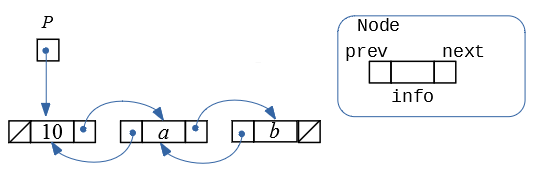
\includegraphics[width=4in]{ds-exam1/nodes.png}}
\caption{\label{fig:nodes} Doubly linked list}
\end{figure}

Variable {\tt P} is a pointer of type {\tt Node*}, 
initially {\tt P} points to the first node in this list. 
The {\tt info} fields in this list have values $10$, $a$ and $b$. 

Write code that modifies this doubly linked list in the following way:
\begin{itemize}
\item If $a > b$, the pointers in the list change so that the \texttt{Node} with \texttt{info} field value $10$ points to $b$ (that \texttt{Node} is now second), and the \texttt{Node} with \texttt{info} field $b$ points to $a$ (that \texttt{Node} is now third). 
\item If $a \leq b$, then your code should leave the list unchanged.
\end{itemize}

%\vfill
%\clearpage


\begin{Verbatim}[frame=single,numbers=left]
int a = P -> next -> info;
int b = P -> next -> next -> info; 
if (a > b) {
    P -> next -> next -> next = P -> next;
	P -> next = P -> next -> next; 
	P -> next -> next -> next = NULL;
	
	P -> next -> prev = P;
	P -> next -> next -> prev = P -> next;
}
\end{Verbatim}


\answer {

The above code snippet could rearrange the nodes. The first 3 assignments under the {\bf if} statement should come in certain order
to avoid information loss. 
If you want to change this order, you might need to introduce some
temporary pointer variables (which is perfectly fine as long as the resulting linked list is not broken).
Figure~\ref{fig:nodes-solution} shows step-by-step process of reassigning pointers. 

\begin{figure}[!htb]
\center{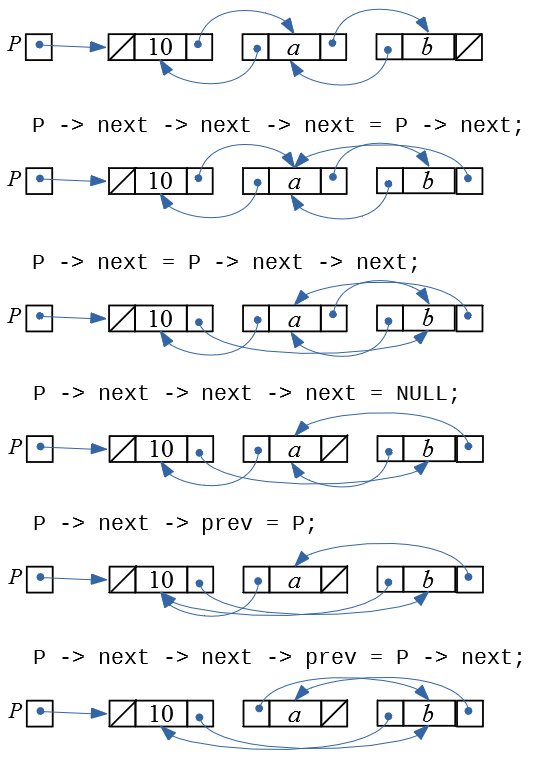
\includegraphics[width=3in]{ds-exam1/nodes-solution.png}}
\caption{\label{fig:nodes-solution} Doubly linked list being rearranged}
\end{figure}


{\bf Note:} We cannot simply reassign {\tt info} fields, since they are constant and do not change over the lifetime of the nodes.
There are some other situations when it is easier to leave the pointers as they are, but swap the contents of 
the {\tt info} fields.
}


\clearpage

%%%%%%%%
%% 03 %%
%%%%%%%%
\item \label{q:q4}
% 4.B. (C++ code) Use STL classes for lists, stacks, queues with iterators.

The following C++ program declares a class {\tt Pair}. 
Pairs are {\em lexicographically ordered}: 
\[
(x_1, y_1) < (x_2, y_2)\ \ \text{iff}\ \ x_1 < x_2\ \vee\ (x_1 = x_2\ \wedge\ y_1 < y_2).
\]
Complete the code below so that, when compiled and executed, in order:
\begin{itemize}
\item a positive integer $n$ is input,
\item $n$ pairs from the standard input are input,
\item the $n$ pairs are pushed on the stack, skipping pairs which are not lexicographically larger than the current top element of the stack,
\item the remaining pairs are output to the standard output as separate lines in their original order.
\end{itemize}

Use the overloaded operators ``{\tt cout << pair}'', ``{\tt cin >> pair}'', ``{\tt p1 < p2}''
for input, output and comparisons. The only data structure to use is STL stack. 
If necessary, you may use several stacks.

\begin{Verbatim}[frame=single,numbers=left]
#include <iostream>
#include <stack>
using namespace std;
class Pair { public: int x; int y; }; 
istream &operator>>(istream  &input, Pair &p ) { 
  input >> p.x >> p.y;   return input;            
}
ostream &operator<<(ostream &output, const Pair &p ) { 
  output << "(" << p.x << "," << p.y << ")";   return output;            
}
bool operator<(const Pair &left, const Pair &right) {
  // implement the lexicographic comparison operator.
}
int main() {
  // Input the total number of pairs, then 2*n integers (the pairs). 
  // Output those pairs which are in lexicographically increasing order.
}
\end{Verbatim}

{\bf Sample input}

\begin{Verbatim}[frame=single]
5
4 17
4 17
5 1000
7 12
7 9
\end{Verbatim}

{\bf Sample output}

\begin{Verbatim}[frame=single]
(4,17)
(5,1000)
(7,12)
\end{Verbatim}



%{\color{blue} 
%\textcolor{blue}{
\answer{
One possible solution is shown below. 
}

{\small
\begin{Verbatim}[frame=single,numbers=left]
#include <iostream>
#include <stack>
using namespace std;
class Pair { 
  public: int x; int y; 
  Pair() { 
    cout << "Default constructor" << endl; 
  }
  Pair(const Pair& arg) { 
    cout << "Copy constructor on (" << x << "," << y << ")" << endl; 
    x = arg.x;
    y = arg.y;
  }
  ~Pair() {
    cout << "Destructor on (" << x << "," << y << ")" << endl; 
  }

}; 
istream &operator>>(istream  &input, Pair &p ) { 
  input >> p.x >> p.y;   return input;            
}
ostream &operator<<(ostream &output, const Pair &p ) { 
  output << "(" << p.x << "," << p.y << ")";   return output;            
}
bool operator<(const Pair &left, const Pair &right) {
  return (left.x < right.x) || (left.x == right.x && left.y < right.y);
}
int main() {
    int n; 
    cin >> n; 
    stack<Pair> myStack;
    for (int i = 0; i < n; i++) {
        Pair p; 
        cin >> p;
        if (myStack.empty() || myStack.top() < p) {
            myStack.push(p);
        }        
    }
    stack<Pair> otherStack;
    while (!myStack.empty()) {
        otherStack.push(myStack.top());
        myStack.pop();
    }    

    while (!otherStack.empty()) {
        cout << otherStack.top() << endl;
        otherStack.pop();
    }    
}
\end{Verbatim}
}

%\clearpage

%%%%%%%%
%% 04 %%
%%%%%%%%
\item 
% 2.B. The order how constructors and destructors are executed.
In your code from Question \ref{q:q4}, define the default (no argument) constructor, copy constructor 
and destructor. Describe the order in which these are called when your compiled code is executed with the input below.

\begin{Verbatim}[frame=single]
2
2 3
1 4
\end{Verbatim}

In your answer you should list the order how the constructors of both types (and also destructor)
are invoked for every {\tt Pair} object. Describe why this behavior makes sense 
and generalize -- how many invokations would happen for $n$ pairs in the input.


\begin{verbatim}
Default constructor
Copy constructor on (8914240,8913088)
Destructor on (2,3)
Default constructor
Destructor on (1,4)
Copy constructor on (8984152,8978256)
Destructor on (2,3)
(2,3)
Destructor on (2,3)
\end{verbatim}

\answer{

A sample order on the calls of constructors/destructors is shown in the above plaintext fragment. 
The first pair $(2,3)$ is constructed three times (first, it is read from the input, then 
added to a stack -- which causes a copy constructor, finally it is also 
copied to another stack to reverse order). 
The second pair $(1,4)$ is skipped (so it is only constructed once). 
For every constructor (either default or copy constructor) there should be one destructor. 

In general, if there are $n$ pairs in the input and $k \leq n$ of these pairs are not skipped, 
then the number of constructor calls would be $3k + (n-k)$ -- namely, every non-ignored
pair is constructed three times, but every ignored pair is constructed just once.

For your implementation the number of constructor calls may differ, but 
some principles should still apply (every constructor has a matching destructor, etc.)
}





\vspace{1cm}

%%%%%%%%
%% 05 %%
%%%%%%%%
\item
% 3.A. Find the asymptotic growth for a given function.

Consider the functions $f_1(n)$, $f_2(n)$, $f_3(n)$, $f_4(n)$ below, mapping positive integers $n \geq 5$
to positive real numbers $t>0$: 
% n^3.5
% 
\begin{align*}
f_1(n) & = (1 + \cos n) \sqrt{2^{7 \cdot \log_2 (n)}},\\
f_2(n) & = 13^{\log_2 (n)},\\
f_3(n) & = \frac{1}{n^2} \cdot {n \choose 5},\\
f_4(n) & = f_1(n) + f_2(n) + f_3(n).
\end{align*}

For each function $f_i(n)$, $i=1,2,3,4$, find functions 
\begin{itemize}
\item $g_i(n)$ such that $f_i(n)$ is $O(g_i(n))$,
\item $h_i(n)$ such that $f_i(n)$ is $\Omega(h_i(n))$, 
\item $k_i(n)$ such that $f_i(n)$ is $\Theta(k_i(n))$. 
\end{itemize}
Give justifications for all your answers.
\end{enumerate}

\answer{

\begin{enumerate}
\item $f_1(n)$ is in $O(n^{3.5})$. To see this, rewrite like this: 
\[ \sqrt{2^{7 \cdot \log_2 (n)}} = \sqrt{(2^{\log_2 (n)})^7} = \sqrt{n^7} = n^{3.5}. \]
Moreover, $f_1(n)$ is in $\Omega(0)$ (in fact, $1 + \cos n$ returns to the value $0$ infinitely often). 
So the bottom estimate of how this function grows cannot be any bigger than $O(0)$.\\
Function $g(n)$ such that $f_1(n)$ is in $\Theta(g(n))$ does not exist (as Big-O and Big-Omega estimates differ). 
\item $f_2(n)$ is in $O(n^{\log_2 13})$ this  (same as $O(n^{3.7})$). Same answer about Big-Omega and Big-Theta.
\item $f_3(n)$ is in $O(n^3)$. This is because ${n \choose 5}$ is the 5th degree polynomial: 
\[ {n \choose 5} = \frac{n(n-1)(n-2)(n-3)(n-4)}{5!}. \]
If you divide 5th degree polynomial by $n^2$, it ends up being $O(n^3)$. Same answer applies for Big-Omega and Big-Theta.
\item $f_4(n)$ is in $O(n^{\log_2 13}) \approx O(n^{3.7})$ (as $\log_2 13$ is the largest exponent among 
all the functions $f_1(n)$, $f_2(n)$, $f_3(n)$, so we can ignore all the smaller exponents, including
the fluctuating $f_1(n)$). 
Same answer for Big-Omega and Big-Theta.
\end{enumerate}

}


\end{document}